\section{\api}

本節では,アクターモデルの振る舞いを強制するために非同期 $\pi$ 計算に型を付けた \api について説明する.
まず \api における\conf の定義をする.次に型システムを導入するが,その際に仮名関数という関数を導入し,型付け規則を定義する.最後にこの型システムにおける健全性について述べる.
また,\api の定義および使われている記号は,文献\cite[Dean2008]{Agha:2004aa} で用いられているものを用いる.

%% \section{準備}

%% これ以降で用いる記号の定義をする.

%% \begin{dfn}[組]
%%   $\tuple{x_1,x_2,...,x_n}$ と書いたとき,これを $x_1, x_2, ..., x_n$ の組 (tuple) とする.単に $\tuple{}$ と書いたときは要素がない組である.

%%   $\tilde{x}$ は名前の組であることを表す.$\{\tilde{x}\}$ と書いたときは,要素として $\tilde{x}$ のみを持つ集合ではなく,$\tilde{x}$ に含まれる名前の集合を表す.また,組を連結する二項演算子を,$\tilde{+}$ と定義する.
%% \end{dfn}

%% \begin{dfn}[要素数が0または1の集合]
%%   空集合であるか,または要素が $z$ のみである集合を $\hat{z}$ と書く.
%%   $\tuple{\hat{z}}$ と書いたときは $\hat{z}$ 一つの組ではなく,$\hat{z} = \emptyset$ であるときは $\tuple{}$ ,$\hat{z} = {z}$ であるときは $\tuple{z}$ とする.
%% \end{dfn}




\subsection{\conf}

%% \conf (configuration)は,アクターシステムのある時点での状態を表す.
\api における\conf の文法は,\srcref{api_config} のようになっている.

\begin{figure}[h]
  \begin{eqnarray}
    P & ::= & \nilconf \mid \actorconf{x}{y}{P} \mid \sendconf{x}{y} \mid \restrictconf{x}{P} \mid \composeconf{P_1}{P_2} \ \nonumber \\
    & & \mid \caseconf{x}{y_1 : P_1 ,..., y_n : P_n} \ \nonumber \\
    & & \mid \instantiate{\tilde{u}}{\tilde{v}}{u_1}{z}{P}{\tilde{x}}{\tilde{y}} \nonumber
  \end{eqnarray}
  \caption{\api の\conf の文法}
  \label{api_config}
\end{figure}

%% \begin{figure}[h]
%%   \begin{align*}
%%     P & ::= \nilconf & \mbox{何もしない} \\
%%     & \mid \actorconf{x}{y}{P} & \mbox{メッセージを受け取って} y \mbox{に束縛し,} P \mbox{を実行する} x \mbox{というアクターを作る} \\
%%     & \mid \bar{x} y & hoge \\
%%     & \mid (\nu x)P & hoge \\
%%     & \mid P1 | P2 & hoge \\
%%     & \mid {\tt case} \ x \ {\tt of} \ (y_1 : P_1 ,..., y_n : P_n) & hoge \\
%%     & \mid B \langle \tilde{x} ; \tilde{y} \rangle & \mbox{振る舞いの雛形} B \mbox{に,}\langle \tilde{x} ; \tilde{y} \rangle \mbox{を使ってアクターを作る}
%%   \end{align*}
%%   \caption{\api の文法}
%%   \label{api_config2}
%% \end{figure}


%% それぞれの説明を以下に示す.
通常の $\pi$ 計算と異なる点は,他のアクター(プロセス)にメッセージを送ったあとにさらに何かを実行できないこと,名前の場合分けが書けること,振る舞いの雛形からアクターを作るための文法があること,の3つである.

%% \begin{description}[style=nextline,leftmargin=50pt]
%%   \item[$\nilconf$]
%%     何もしない.
%%   \item[$\actorconf{x}{y}{P}$]
%%     $(y).P$ という振る舞いを持つアクター $x$ をつくる.ここで振る舞いとは,$y$ というメッセージを受け取って $P$ を実行するという意味である.
%%   \item[$\sendconf{x}{y}$]
%%     $x$ という名前のアクターに $y$ という名前を送る.
%%   \item[$\restrictconf{x}{P}$]
%%     $P$ 中に現れる $x$ という名前を環境から隠す.
%%   \item[$\composeconf{P1}{P2}$]
%%     $ P1 $ と $ P2 $ を並列に実行させる.
%%   \item[$\caseconf{x}{y_1 : P_1 ,..., y_n : P_n}$]
%%     名前 $x$ が $y_i$ と一致したとき $ P_i $ を実行する.一致するものが複数ある場合は,そのなかから非決定的に選ばれたものを実行する,一致するものがない場合は $0$ になる.
%%   \item[$\instantiate{\tilde{u}}{\tilde{v}}{u_1}{z}{P}{\tilde{x}}{\tilde{y}}$]
%%     振る舞いの雛形である $\behaviortemplate{\tilde{u}}{\tilde{v}}{u_1}{z}{P}$ に,$(\tilde{x}, \tilde{y})$ を与えてアクターを作る.ただし $len(\tilde{x}) = len(\tilde{u}), len(\tilde{y}) = len(\tilde{v})$ かつ $\tilde{x}$ は要素数が1または2の組であり,$x_1$ は $\tilde{x}$ の1番目の要素である.例えば,$\instantiate{\tuple{u}}{\tuple{v}}{u}{z}{\sendconf{v}{z}}{\tuple{x}}{\tuple{y}}$ は,$\actorconf{x}{z}{\sendconf{y}{z}}$ となる.
%% \end{description}


\subsection{型システムの導入}

\api の文法のみでは,アクターモデルの性質は満たさないような\conf も書けてしまう.例えば,$x(u).P | x(v).Q$ は \api の文法で書けるが,$x$ という名前のアクターが2つ作られるので,\unique を満たしていない.また,$x(u).(u(v).P | x(v).Q)$ も \api の文法で書けるが,メッセージとして送られてきた名前でアクターが作られているので,\fresh に反する.

また,アクターモデルでは,1回の通信で複数の名前を送信することができるが,\api では1回の通信で一つの名前しか送ることはできない.複数の名前を送信するには,その数だけ連続して通信する必要がある.
しかし,アクターモデルではこのような複数の名前を含むメッセージの受け渡しはアトミックに行なわれ,即座に次のメッセージを受け取れる状態にならなければいけない.
そこで,いつでもメッセージを送信できるという永続性を弱め,アクターはメッセージの送信先のアクターの処理が終わるまで待てるようにする(いつかは必ず送れる).そしてアトミックに行うことのできない処理の最中はメッセージを送れないということを,正規の名前を隠して一時的な名前を使って処理を行うことで実現させる.
ここで,仮の名前をとった後,元の名前とは異なる名前になってしまうと,そのアクターにメッセージを送ろうとしているアクターはメッセージを送れなくなってしまい,永続性に反する.仮の名前をとったときには必ず元の名前に戻るという制約が必要である.

以上のような性質を満たすようにするため,型システムを導入し,\api に制約を与える.


%% アクターがなんらかの処理を行っているときには,終わるまで待つようにし,処理中はメッセージを受けつけられないように,一時的な名前でもって処理を行うことで実現させる.
%% 他のアクターからのメッセージを受け付けないようにするため一時的な名前でもって処理を行うこととする.
%% ただし,処理中のアクターにメッセージを送信したいアクターは,その処理が終わり元の名前に戻るまで待たなければならなくなる.これはいつでもメッセージを送信できるという永続性に反するが,ここでは永続性を,必ず送ることはできるが待つ必要がある可能性がある,というものに弱める.

%% 例えば,\api では

%% しかし,この変換では,すべての名前を送受信し終わるまで待つ必要があり,これは.
%% このような,2つのアクターが同期する必要があるタスクは,以下のように一時的な名前をとってその名前を用いて行うようにする.

%% \begin{center}
%%   $\bar{x} \langle y_1,..., y_n \rangle = (\nu u)(\bar{x} u | u(z).(\bar{z} y_1 | u(z).(\bar{z} y_2 | ... | u(z).(\bar{z} y_n) ... )))$ \\
%%   $x(y_1, ... , y_n).P = x(u).(\nu z)(\bar{u} z | z(y_1).(\bar{u} z | z(y_2).(\bar{u} z | ... | z(y_n).(\bar{u} z | P)...)))$ \\
%% \end{center}

%% 2つの名前に限定すれば,これは以下のようになる.

%% \begin{center}
%%   $\bar{x} \langle y_1, y_2 \rangle = (\nu u)(\bar{x} u | u(z).(\bar{z} y_1 | u(z).\bar{z} y_2))$

%%   $x(y_1, y_2).P = x(u).(\nu z)(\bar{u} z | z(y_1).(\bar{u} z | z(y_2).(\bar{u} z | P)))$ \\
%% \end{center}

%% ここで,仮の名前をとった後,元の名前とは異なる名前になってしまうと,そのアクターにメッセージを送ろうとしているアクターはメッセージを送れなくなってしまい,永続性に反する.仮の名前をとったときには必ず元の名前に戻るという制約が必要である.

%% 以上のような性質を満たすようにするため,型システムを導入し,\api に制約を与える.


%% また,アクターモデルでは,1回の通信で複数の名前を送信することができるが,\api では1回の通信で一つの名前しか送ることはできない.
%% $\pi$ 計算も同様に1回の通信で一つのメッセージしかおくることはできないが,以下のようにエンコードすることによって,複数の名前を送るようにできる.


%% \begin{center}
%%   $\bar{x} \langle y_1,...,y_n \rangle .P = (\nu w)\bar{x}w.\bar{w}y_1. \ ... \ .\bar{w}y_n.P$ \\
%%   $x(y_1,...,y_n).P = x(w).w(y_1). ... .w(y_n)$
%% \end{center}


%% しかし,\api では $pi$ 計算とは異なり,メッセージを送ったのち動作を続けることはできない.\api では,以下のようにエンコードする.

%% \begin{center}
%%   $x(y_1, ... , y_n).P = x(u).(\nu z)(\bar{u} z | z(y_1).(\bar{u} z | z(y_2).(\bar{u} z | ... | z(y_n).(\bar{u} z | P)...)))$ \\
%%   $\bar{x} \langle y_1,..., y_n \rangle = (\nu u)(\bar{x} u | u(z).(\bar{z} y_1 | u(z).(\bar{z} y_2 | ... | u(z).(\bar{z} y_n) ... )))$
%% \end{center}

%% 2つの名前に限定すれば,これは以下のようになる.

%% \begin{center}
%%   $\bar{x} \langle y_1, y_2 \rangle = (\nu u)(\bar{x} u | u(z).(\bar{z} y_1 | u(z).\bar{z} y_2))$

%%   $x(y_1, y_2).P = x(u).(\nu z)(\bar{u} z | z(y_1).(\bar{u} z | z(y_2).(\bar{u} z | P)))$ \\
%% \end{center}


%% 以上のような性質を満たすようにするため,型システムを導入し,\api に制約を与える.


\subsubsection{\tmp}



%% \tmp (temporary name mapping function)

%% \note{なぜ \tmp が必要なのか}

%% アクターモデルでは,一つのメッセージで組として複数の名前を送信することができる.しかし,\api ではひとつのメッセージに一つの名前しか送信することができない.

%% また,アクターモデルではメッセージを受け取って何らかの行動をとる,という振る舞いがアトミックに行われる.しかし,\api ではメッセージを受け取るという行動と何らかの行動をとるという行動に分離されていて,アトミックには行われない.

%% \api は一度の通信で一つのメッセージ(名前)しか送ることができない.しかし,アクターモデルは複数の名前の送信をアトミックに行えなければいけない.




%% 複数のメッセージをすべて終わるまで待つというようになってしまって,他のメッセージを受け取れなくなる.
%% しかし永続性があるので,送信側のアクターも受信側のアクターも,メッセージを受信できなければ(readyでなければ)いけない.



%% したがって,永続性が必要とする条件を弱めることにする.メッセージを受け取った後新しい振る舞いに変わる代わりに,同期状態になる(次のメッセージが来る前)まで待つことができるようにする.

%% 仮の名前をとれるようにする.

%% 基本的に,同期する必要があるタスクは仮の名前に任せられ,終わったら元の正規の名前に戻る.

%% \note{とても例欲しい}


%% 複数の名前を送信するとき,仮の名前をとっていた.

%% アクターモデルでは非同期的にメッセージのやりとりが行われるが,\api のメッセージのやりとりは同期的に行われる.複数の名前を送信する状況を考えると,一回の同期で通信を終えなければならない.
%% 通信中のアクターにメッセージを送りたいときは,すべてのメッセージが送受信されるまで待たなければいけないが,これはアクターモデルの性質である\persist に反している.\api では,\persist の制限を緩め,メッセージを送受信できる状態になるまで待てるようにする.
%% 通信中のアクターにメッセージを送れるとだめである.よって,同期してメッセージを送受信するときは,アクターは仮の名前をとり,その名前でタスクを実行し,そのタスクが終わったら元の正規の名前に戻る.


%% 通信しているアクターにメッセージを送信したいアクターは待たなければいけない.

%% これは\persist に違反しているが,この部分の\persist は許すことにする.



%% 上述したような,複数の名前を通信するような同期が必要となるタスクは,一時的な名前を用いて行い,タスクが終わると元の名前に戻るようにする.

仮の名前は必ず正規の名前に戻るという制約を型システムを用いて与えるためには,仮の名前をとったときに正規の名前を覚えておく必要がある.そこで仮の名前から元の正規の名前にマッピングする関数を導入する.これを \tmp (temporary name mapping function) と呼ぶ.

\begin{dfn}[\tmp]
  \tmp $f$ は,集合 $X$ から集合 $X^*$ への写像である.
  ただし,${\cal N}$ を名前全体の集合として,$ \bot, \ast \notin {\cal N}, X \subset {\cal N}, X^* = X \cup \{\bot,\ast\} $ である.
\end{dfn}

\tmp は以下の通り定義される.

\begin{table}[htb]
  \begin{tabular}{ll}
    $ f(x) = \bot $ & $ x $ が正規の名前のとき \\
    $ f(x) = \ast $ & $ x $ が環境から隠されている \\
    & 名前であるとき \\
    $ f(x) = y \notin \{\bot,\ast\} $ & アクター $ y $ の仮の名前が \\
    & $ x $ であるとき
  \end{tabular}
\end{table}

また,$f^{*} : X^* \rightarrow X^*$ を以下のように定義する.

\begin{adjustvboxheight}
  \[ f^{*}(x) = \begin{cases}
    f(x) & x \in X \mbox{のとき} \\
    \bot & x = \ast \mbox{\ または} x = \bot \mbox{\ のとき}
  \end{cases} \]
  \vspace{1pt}
\end{adjustvboxheight}


\subsubsection{\tmp の構築}

\tmp は以下に示す $ch$ 関数,\tmp の合成,\tmp の制限のいずれかで作ることができる.

\begin{dfn}[$ch$]
  $ch$ は名前の組をとり,\tmp を返す関数である.組の長さは任意である.組を $\tuple{x_1,x_2,...,x_n}$ としたとき,$ch(\tuple{x_1,x_2,...,x_n})$ は以下のような\tmp となる.\\
\begin{adjustvboxheight}
  \[ ch(\tuple{x_1,x_2,...,x_n})(x_i) = \begin{cases}
    x_{i + 1} & 1 \leq i < n \mbox{のとき} \\
    \bot & i = n \mbox{のとき}
  \end{cases} \]
  \vspace{1pt}
\end{adjustvboxheight}
\end{dfn}



\begin{dfn}[\tmp の合成]
  $f_1 : \rho_1 \rightarrow \rho_1^*$,$f_2 : \rho_2 \rightarrow \rho_2^*$ とする.
  \tmp の合成を表す二項演算子 $f_1 \oplus f_2 : \rho_1 \cup \rho_2 \rightarrow (\rho_1 \cup \rho_2)^*$ を以下のように定義する.\\
\begin{adjustvboxheight}
  \[ (f_1 \oplus f_2)(x) = \begin{cases}
    f_1(x) & x \in \rho_1 \mbox{かつ} f_1(x) \neq \bot \mbox{,また} \\
    & \mbox{は} x \in \rho_1 \mbox{かつ} x \notin \rho_2 \mbox{のとき} \\
    f_2(x) & \mbox{その他}
  \end{cases} \]
  \vspace{1pt}
\end{adjustvboxheight}
\end{dfn}


\begin{dfn}[\tmp の定義域の制限]
  $f : \rho_1 \rightarrow \rho_1^*, \rho \subset \rho_1$ である $f, \rho$ に対して定義域の制限を表す二項演算子 $f | \rho : \rho \rightarrow \rho^*$ を以下のように定義する. \\
\begin{adjustvboxheight}
  \[ (f | \rho)(x) = \begin{cases}
    f(x) & f(x) \in \rho \mbox{のとき} \\
    \ast & \mbox{その他}
  \end{cases} \]
  \vspace{1pt}
\end{adjustvboxheight}
\end{dfn}


\subsubsection{\tmp が満たすべき性質}

\tmp $f$ はその定義から,以下を満たすべきである.

\begin{itemize}
  \item $ f(x) \neq x $
  \item $ f(x) = f(y) \notin \{\bot,\ast\} \Rightarrow x = y $
  \item $ f^{*}(f(x)) = \bot $
\end{itemize}

$ f(x) \neq x $ は,仮の名前から正規の名前を得たとき,それは仮の名前と同名ではないという性質である.
$ f(x) = f(y) \notin \{\bot,\ast\} \Rightarrow x = y $ は,正規のアクターは2個以上の仮の名前をとれないという性質である.
$ f^{*}(f(x)) = \bot $ は,仮名のアクターはさらに仮の名前を持つことはできないという性質である.

また,互換性という性質を定義する.

\begin{dfn}[互換性(compatible)]
  二つの\tmp $f_1, f_2$ が以下の性質を満たすとき,$f_1,f_2$ は互換性を持つという.また,この性質を満たすという述語を $compatible(f_1,f_2)$ と書く.
  \begin{itemize}
    \item $f_1 \oplus f_2 = f_2 \oplus f_1$
    \item $f_1 \oplus f_2$ が\tmp の性質を満たす
  \end{itemize}
\end{dfn}

\subsection{型付け規則}

\api が先に述べた性質を満たすようにするための型付け規則は \srcref{api:typing} のようになっている.\conf $ P $ ,$ P $ の\recep $ \rho $ ,$ P $ 中の仮の名前から正規の名前への写像 $f : \rho \rightarrow \rho^*$ で, $\rho ; f \vdash P$ が成り立つとき,$ P $ は正しく型付けされている.

\begin{figure*}[t]
  \infrule[Nil]{
  }{
    \typing{\emptyset}{\{\}}{\nilconf}
  }
  \vspace{14pt}
  \infrule[Msg]{
  }{
    \typing{\emptyset}{\{\}}{\sendconf{x}{y}}
  }
  \vspace{14pt}
  \infrule[Act]{
    \typing{\rho}{f}{P}
    \andalso \rho - \{x\} = \hat{z}
    \andalso y \notin \rho
    \andalso f = \begin{cases}
      ch(\tuple{x} \tupapp \tuple{\hat{z}}) & x \in \rho \mbox{のとき} \\
      ch(\tuple{\hat{z}}) & \mbox{その他}
    \end{cases}
  }{
    \typing{\{x\} \cup \hat{z}}{ch(\tuple{x} \tupapp \tuple{\hat{z}})}{\actorconf{x}{y}{P}}
  }
  \vspace{14pt}
  \infrule[Case]{
    \forall 1 \leq i,j \leq n , i \neq j, \ \typing{\rho_i}{f_i}{P_i}
    \andalso compatible(f_i, f_j)
  }{
    \typing{(\cup_i \rho_i)}{(f_i \oplus f_2 \oplus ... \oplus f_n)}{
      {\tt case} \ x \ {\tt of} \ (y_1 : P_1,...,y_n : P_n)
    }
  }
  \vspace{14pt}
  \infrule[Comp]{
    \typing{\rho_1}{f_1}{P_1}
    \andalso \typing{\rho_2}{f_2}{P_2}
    \andalso \rho_1 \cap \rho_2 = \phi
  }{
    \typing{\rho_1 \cup \rho_2}{f_1 \oplus f_2}{P_1 | P_2}
  }
  \vspace{14pt}
  \infrule[Res]{
    \typing{\rho}{f}{P}
  }{
    \typing{\rho - \{x\}}{f|(\rho - \{x\})}{\restrictconf{x}{P}}
  }
  \vspace{14pt}
  \infrule[Inst]{
    \typing{\{\tilde{u}\}}{ch(\tilde{u})}{\actorconf{u_1}{z}{P}}
    \andalso len(\tilde{x}) = 2 \ \Rightarrow \ x_1 \neq x_2
  }{
    \typing{\{\tilde{x}\}}{ch(\tilde{x})}{\instantiate{\tilde{u}}{\tilde{v}}{u_1}{z}{P}{\tilde{x}}{\tilde{y}}}
  }

  \caption{型付け規則}
  \label{api:typing}
\end{figure*}

%% それぞれの規則についての説明を以下に示す.

%% \begin{description}[style=nextline,font=\normalfont\scshape]
%%   \item[Nil]
%%     $\nilconf$ 中にはアクターは存在しないので,\recep は空集合,\tmp は空関数で型付けできる.

%%   \item[Msg]
%%     $\sendconf{x}{y}$ 中にはアクターは存在しないので,\textsc{Nil} と同様に\recep は空集合,\tmp は空関数で型付けできる.

%%   \item[Act]
%%     $y \notin \rho$ は,メッセージの名前でアクターを作れないということを表しているため,これがあることで\fresh が保証される.
%%     また,$\hat{z} = \{z\}$ であるときは,$z$ は $x$ を一時的な名前としてとっていることを表しており,$\hat{z} = \emptyset$ であるときは,$x$ がアクターの正規の名前であることを表している.

%%   \item[Case]
%%     相互に互換性を持つという条件によって,一つのアクターが複数の仮の名前を持つということが起こらないことを保証している.

%%   \item[Comp]
%%     $\rho_1 \cap \rho_2 = \phi$ から,\unique が保証される.

%%   \item[Res]
%%     $P$ 中に現れるアクター $x$ を外部から隠すので,\recep から $\{x\}$ を引き,\tmp も制限している.

%%   \item[Inst]
%%     $len(\tilde{x}) = 2$ であるときは,$x_1$ は $x_2$ の仮の名前であることを表している.また,$x_1 \neq x_2$ という条件によって,仮の名前が正規の名前と同名にならないようにしている.
%%     $len(\tilde{x}) = 1$ であるときは,$x_1$ は正規の名前である.
%% \end{description}

\subsection{型システムの健全性}

\api の型システムにおける健全性は,この型システムを満たした \api の\conf はアクターモデルとしての振る舞いを示すということを表した性質である.
単純型付きλ計算における型システムの健全性のような,正しく型付けされるならば stuck 状態にならないという性質とは少し異なることに注意されたい.

\api の型システムの健全性は以下のように定義されている.

\begin{thm}[\api の健全性]
  \conf $P$ について,$\typing{\rho}{f}{P}$ で型付けできたとき,{\rm 以下の3つの性質を満たす.}

  \begin{itemize}
  \item
    $\rho$ は $P$ 中に現れる\free の部分集合である {\rm (\recep の健全性)}
  \item
   {\rm  以下の3つを満たす (仮名の取り方の健全性)}
    \begin{enumerate}
      \item $ f(x) \neq x $
      \item $ f^{*}(f(x)) = \bot $
      \item $ f(x) = f(y) \neq \{\bot, \ast\} \Rightarrow x = y $
    \end{enumerate}
  \item
    $\typing{\rho'}{f'}{P}$ ならば, $\rho = \rho'$ かつ $f = f'$ {\rm (型付けの一意性)}
  \end{itemize}
\end{thm}

それぞれは以下の意味を持っている.

\begin{description}[style=nextline]
  \item[\recep の健全性]
    \recep に属するアクターはメッセージとして送られてきた名前で作られたものではなく,かつ環境から隠されたものでもない.
  \item[仮名の取り方の健全性]
    アクターが仮の名前をとったとき,それは同名のものではなく,さらに仮の名前を持つこともない.また,アクターが複数の仮の名前を持つことはない.
  \item[型付けの一意性]
    \conf に型が付いたとき,その型付けは一意である.
\end{description}


%% \api は以下の定理が成り立つ.

%% \begin{thm}[]
%%   \api の型システムは健全である.
%% \end{thm}

%% \begin{thm}[\api の健全性]


%%   \begin{lem}[\api の\recep]
%%     $\rho \subset fn(P)$
%%   \end{lem}

%%   \begin{lem}[\api の\tmp の性質]
%%     \begin{enumerate}
%%       \item $ f(x) \neq x $
%%       \item $ f^{*}(f(x)) = \bot $
%%       \item $ f(x) = f(y) \neq \{\bot, \ast\} \Rightarrow x = y $
%%     \end{enumerate}
%%   \end{lem}

%%   \begin{lem}[型付けの一意性]
%%     $\typing{\rho'}{f'}{P}$ ならば, $\rho = \rho'$ かつ $f = f'$
%%   \end{lem}
%% \end{thm}

%% %% \note{なぜこれが健全性になるのか}
%% %% 何に対しての健全性?

%% %% 当然,\recep は P 中に含まれるbounded name ではいけない.

%% %% Actor Model の性質を満たす.
%% %%   - アクターの名前は一意
%% %%   -


%% \section{並列更新アルゴリズム}\label{section:update}

%% 本節では,後続の操作をブロックしない${\it update\/}$操作を与える.基本的な
%% アイデアは,zig-zigとzig-zagの両方について,目標節点をその深さの
%% 半分までしか浮上させない半扁平化(semi-splaying)を用いることである(文献
%% \cite{ST85}の半扁平化は,zig-zigのみが扁平化と異なっていた).$x$を更新対
%% 象の節点とすると,アルゴリズムは以下のようになる.
%% %
%% % ここでも左右対称な操作の片方のみを述べる.

%% \begin{itemize}
%% % \medskip\noindent (a)
%% \item[(a)]
%% 空の木に対する挿入は図\ref{figure:update}
%% (a1)の操作,(空でない)木の根に対する更新は
%% 図\ref{figure:update}(a2)の操作を行なう.

%% % \begin{adjustvboxheight}
%% \begin{figure*}[t]
%%   \centerline {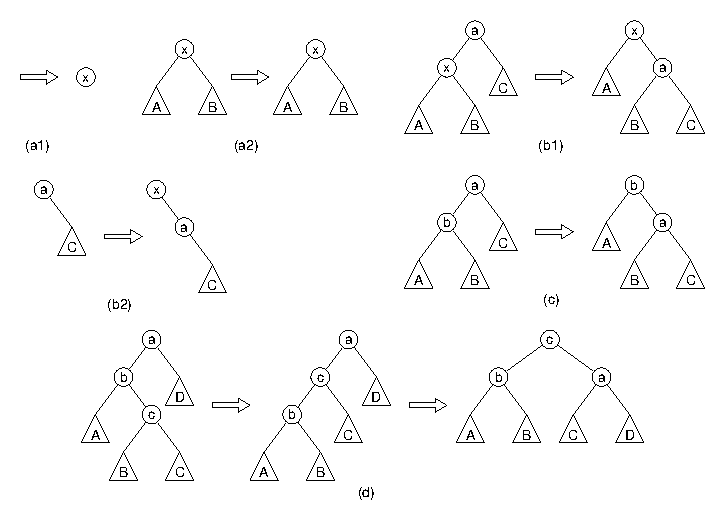
\includegraphics {images/fig3.eps}}
%% \caption{後続操作をブロックしない更新アルゴリズムの1ステップ}
%% \label{figure:update}
%% \end{figure*}
%% % \end{adjustvboxheight}

%% % \medskip\noindent (b)
%% \item[(b)]
%% zig:
%% $x$が左部分木の根である場合は図\ref{figure:update}(b1)
%% の操作,$x$が存在すべき左部分木が空の
%% 場合は図\ref{figure:update}(b2)の操作を行なう.

%% % \medskip\noindent (c)
%% \item[(c)]
%% zig-zig: 図\ref{figure:update}(c)左の木における$x (<b)$の探索では,
%% 枝$ba$の右回転を行なってアクセスしたパスの長さを1短縮する.次は1レベル
%% (短縮前の長さでは2レベル)下降して,部分木$A$に対して再帰的に探索を行なう.

%% % \medskip\noindent (d)
%% \item[(d)]
%% zig-zag: 図\ref{figure:update}(d)左の木における節点$x$ ($b<x<a$) の
%% 探索では,
%% 枝$cb$の左回転と,できた枝$ca$の右回転を行ない,
%% アクセスしたパスを1短縮する.
%% %
%% % 二つの中側の部分木の適当な方に対して再帰的に探索を行なう.
%% %
%% % \noindent
%% $x=c$ならばこれで探索終了である.$x<c$ならば2レベル(短縮前の長さでは3レ
%% ベル)下降して$B$の中から$x$を再帰的に
%% 探索する.$x>c$ならば同様に$C$の中から再帰的に探索する.$x\ge c$の場合には
%% 枝$ca$の回転操作を省略することも考えられる.
%% %
%% $b$の右部分木が空の場合は,そこに節点$x$を挿入
%% したあと,上に述べた回転操作を行なう.

%% \end{itemize}
%% % \medskip
%% 以上の操作で,アクセスしたパスの長さは最悪でも約$2/3$になる.
%% %
%% 半分でなくて$2/3$なのは,上記zig-zag操作の性質によるものである.
